\section {Leave one out cross validation}
\subsection{Theory}
The Leave one out cross validation works a lot like Validation set approach but instead of spliting the data set into two subsets of
similar size, a single observation $(x_1, y_1)$ is used for the testing set and the remaining observations ${(x_2, y_2), . . . , (x_n, y_n)}$ make up the training set and repeat this process as seen in Figure \ref{fig:loocv}.
\begin{figure}[H]
	\centering
	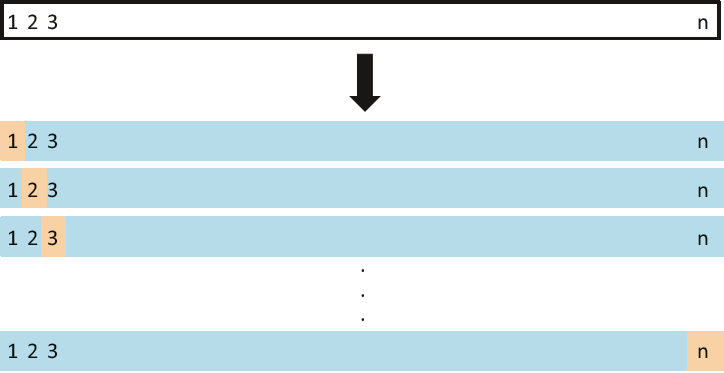
\includegraphics[width=0.5\linewidth]{crossValidation/LOOCV}
	\caption{}
	\label{fig:loocv}
\end{figure}
Repeating this method n times gives n squared errors, $MSE_1, . . . , MSE_n$. The LOOCV estimate for the test MSE is the average of these n test error as shown in equation \ref{fo:LOOCV}.
\begin{align}\label{fo:LOOCV}
CV_{(n)} = \frac {1}{n} \sum_{k=1}^{K}  (\frac {y_i-\hat{y_i}}{1- h_i})^2
\end{align}
Leave one out cross validation has a some advantages over the validation set approach. It has far less bias. Because in LOOCV repeatedly fit the chosen learning method using training sets that contain n - 1 observations that is nearly as many as are in the entire data set. On the other hand the validation set approach training set is typically around half the size of the original data set hence LOOVC won't overestimate the test error rate as much as the validation set approach would. The LOOCV will also give consistent results because there is no randomness in the training/testing set splits and is usefull when there is limited amount of data.

\subsection{Result}
In lab 3.4.2 the same Auto data as used in the validation Set Approach. Running the iteratively LOOCV process for different fits polynomial regressions for polynomials of 1 to 5 and displaying the associated cross-validation error. The output below shows see a drop in the estimated test MSE between the linear and quadratic fits. But using higher-order polynomials shows no clear improvement.
\begin{lstlisting}[language=Python]
24.23151351792922, 19.24821312448969, 19.334984064109666, 19.42443031091358, 19.0332089609506
\end{lstlisting}
When running the LOOCV a mass increased computing time in the machine has seen and that was expected.